We evaluated Damaris with the CM1 atmospheric simulation~\cite{bryan2002benchmark} and ANL's Nek5000 CFD solver~\cite{nek5000}, 
on several platforms: NICS's Kraken~\cite{kraken}, three clusters of the French Grid'5000 platform~\cite{grid5000}, NCSA's BluePrint cluster
and the Blue Waters supercomputer~\cite{bluewaters}. In the following, we first 
evaluate Damaris in the context of improving I/O performance by hiding the I/O variability.
We then evaluate the use of Damaris for several other data management tasks, including data compression, 
I/O scheduling and in situ visualization.

\subsection{Addressing the I/O Bottleneck with Damaris}\label{sec:expIO}

In this first evaluation part, we show how Damaris is used to improve I/O performance.

\subsubsection{Description of the Applications}

The following applications were used in our experiments.
%\begin{SCfigure}[50]
%    \fbox{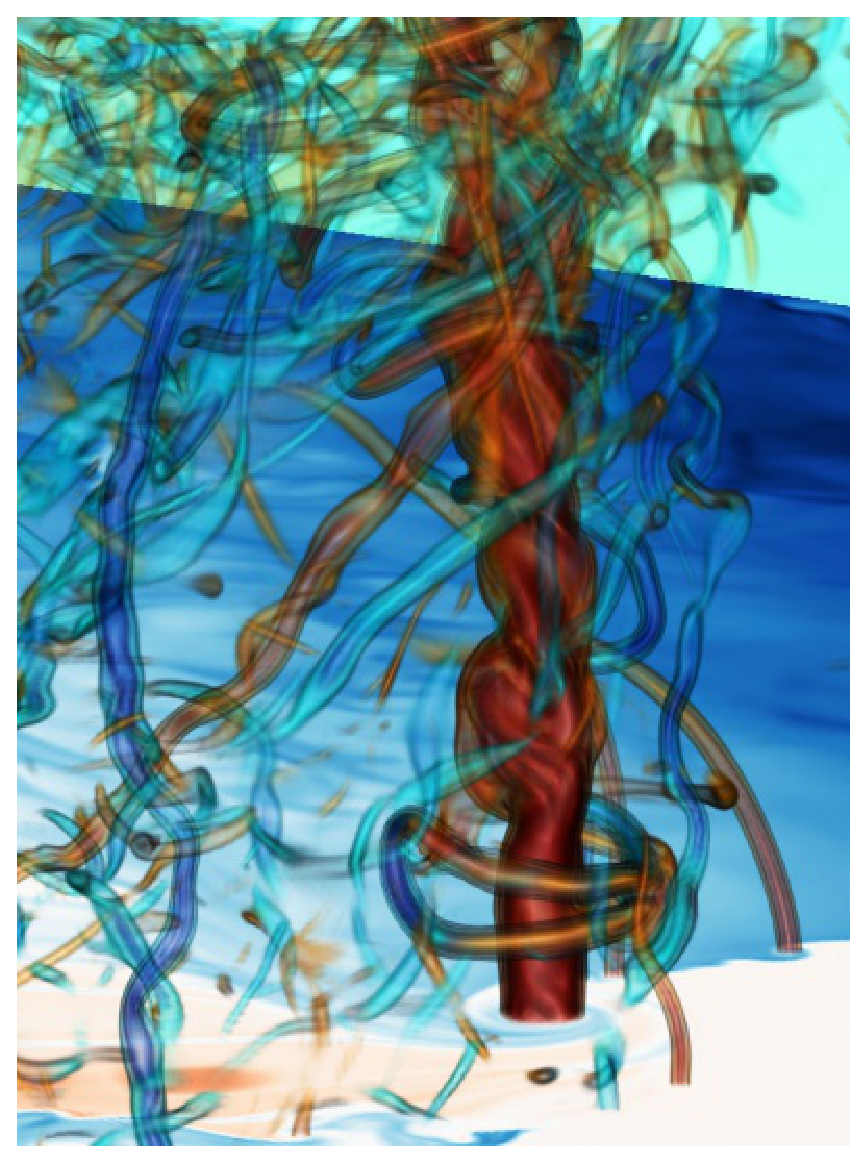
\includegraphics[width=0.38\textwidth,height=0.38\textwidth]{figures/cm1.eps}}
%  \caption[Simulation of a supercell producing a long-track EF5 tornado]{Simulation of a supercell producing a long-track EF5 tornado. 
%  This simulation was realized on NCSA's Blue Waters supercomputer by Leigh Orf (Central Michigan University) 
%  and Bob Wilhelmson (NCSA) using the CM1 code. See~\cite{isgtw-cm1}.}
%\end{SCfigure}

\begin{description}
\item{\textbf{CM1 (Cloud Model 1)}} is used for atmospheric research and is suitable
for modeling small-scale atmospheric phenomena such as thunderstorms
and tornadoes. It follows a typical behavior of scientific simulations,
which alternate computation phases and I/O phases. The simulated domain
is a regular 3D grid representing part of the atmosphere. 
Each point in this domain is characterized by a set of
variables such as local \emph{temperature} or \emph{wind speed}.
CM1 is written in Fortran 90. Parallelization is done using MPI, by
distributing the 3D array along a 2D grid of equally-sized subdomains, each of which
is handled by a process. 
The I/O phase leverages either HDF5 to write one file per
process, or pHDF5~\cite{chilan2006parallel} to write in a shared file in a collective manner.
One of the advantages of using a file-per-process approach is
that compression can be enabled, which cannot be done with pHDF5.
However, at large process counts, the file-per-process approach
generates a large number of files, making all subsequent analysis tasks
intractable.

\item{\textbf{Nek5000}} is a computational fluid dynamics solver based on 
the spectral element method. It is actively developed at ANL's Mathematics 
and Computer Science Division. 
It is written in Fortran 77 and solves its governing equations on an 
unstructured mesh. This mesh consists of multiple 
elements distributed across processes; each element is a small curvilinear mesh.
Each point of the mesh carries
the three components of the fluid's local velocity, as well as other variables.
We chose Nek5000 for this particular meshing structure, different from CM1,
and for the fact that it is substantially more memory-hungry than CM1.
We modified Nek5000 in order to pass the mesh elements and fields data to Damaris.

Nek5000 takes as input the mesh on which to solve the equations, along with 
initial conditions. We call this set a \emph{configuration}. In our
experimental evaluation, we used the \emph{MATiS} configuration, which was
designed to run on 512 to 2048 cores. Another configuration, \emph{turbChannel},
is used in Section~\ref{sec:insitu} to evaluate in situ visualization. This configuration was
designed to run on 32 to 64 cores.
\end{description}

\subsubsection{Platforms and Configurations}

With the CM1 application, our goal was to optimize CM1's I/O for future use on the 
upcoming Blue Waters Petascale supercomputer. Therefore we started with NCSA's IBM Power5 BluePrint 
platform as it was supposed to be representative of Blue Waters' hardware.
On this platform, we evaluated the scalability of the CM1 application with respect to the size of its output, with the file-per-process and 
Damaris approaches. We then experimented on the \emph{parapluie} cluster of Grid'5000's Rennes site.
This cluster features 24-core nodes, which makes it very suitable to our approach based on dedicated cores. 
We then moved our experiments to NICS's Kraken supercomputer, which, in addition to allowing runs at much larger scales, 
has a hardware configuration very close to that of Blue Waters' final design.

With Nek5000, our goal was to confirm the usability of Damaris with a more memory-hungry application.
We completed our experimentation on the \emph{stremi} cluster of Grid'5000's Reims site, which provides the same type
of hardware as the \emph{parapluie} cluster, but a different network.
All these platforms are detailed hereafter, along with the configuration of CM1 and Nek5000 we used.

\begin{description}
\item{\textbf{BluePrint}} is a test platform used at NCSA until 2011 when IBM was still in charge of
delivering the Blue Waters supercomputer.\footnote{As IBM terminated its contract with NCSA in 2011 
and Blue Waters was finally delivered by Cray, BluePrint was later decommissioned and replaced with a 
test platform, JYC, matching the new Blue Waters' design.}
BluePrint features 120 Power5 nodes. Each node consists of 16 cores and 
includes 64~GB of memory. As for its file system, GPFS is deployed on 2 I/O servers.
CM1 was run on 64 nodes (1024 cores), with a $960\times960\times300$-point
domain. Each core handles a $30\times30\times300$-point subdomain with the 
standard approaches, that is, when no dedicated cores are used. 
When dedicating one core out of 16 on each node, computation
cores handle a $24\times40\times300$-point subdomain. On this platform we 
vary the number of variables that CM1 writes, resulting in different sizes of the output.
We enabled the compression feature of HDF5 for all the experiments done on this platform.

\item{\textbf{Grid'5000}} is a French grid testbed. We use its \emph{parapluie} cluster
on the Rennes site and its \emph{stremi} cluster on the Reims site.
On the Rennes site, the parapluie cluster featured 40 nodes of 2~AMD 1.7~GHz CPUs, 12~cores/CPU, 48~GB RAM.
We run CM1 on 28 nodes (672 cores) and 38 nodes (912 cores).
We deployed a PVFS file system on 15 separate I/O servers (2~Intel 2.93~GHz CPUs,
4~cores/CPU, 24~GB RAM, 434~GB local disk). Each PVFS node was
used both as I/O server and metadata server. All nodes (including the file system's) communicate
through a 20G InfiniBand 4x QDR link connected to a common Voltaire switch. 
We use Mpich~\cite{mpich} with ROMIO~\cite{thakur1999data}
compiled against the PVFS library, on a Debian operating system.
The total domain size in CM1 is $1104\times1120\times200$ points, so each core 
handles a $46\times40\times200$-point subdomain with a standard approach, 
and a $48\times40\times200$-point subdomain when one core out of 24 is used by Damaris.

On the Reims site the \emph{stremi} cluster features the same type of node as the \emph{parapluie} cluster.
We run Nek5000 on 30 nodes (720 cores). We deploy PVFS on 4 nodes of the same cluster. Each
PVFS node is used both as I/O server and metadata server. All nodes communicate through a
1G Ethernet network.
We use the MATiS configuration of Nek5000, which contains 695454 elements (small $4 \times 2 \times 4$ curvilinear sub-meshes).
These elements are distributed across available simulation processes. Thus the total number
of elements (and thus the total amount of data output) does not vary whether we use dedicated cores or not.
When no dedicated cores are used, each core handles 965 or 966 such elements. When dedicating one
core out of 24, each simulation core handles 1007 or 1008 elements.

\item{\textbf{Kraken}} is a supercomputer deployed at NICS. It was ranked $11^{th}$ in the 
Top500~\cite{top500} at the time of the experiments, with a peak Linpack performance of 919.1~Teraflops.
It features 9408 Cray XT5 compute nodes connected through a Cray 
SeaStar2+ interconnect and running Cray Linux Environment (CLE). 
Each node has 12 cores and 16~GB of local memory.
Kraken provides a Lustre file system using 336 block storage devices managed
by 48 I/O servers and one metadata server.

On this platform, we studied the weak scalability of the file-per-process,
collective I/O and Damaris approaches in CM1,
that is, we measured how the run time varies with a fixed amount of data per node.
When all cores in each node are used by the simulation, each client process handles a 
$44\times44\times200$-point subdomain.
Using Damaris, each client process (11 per node) 
handles a $48\times44\times200$-point subdomain, which makes the total problem 
size equivalent for a given total number of cores.

\end{description}

\subsubsection{How Damaris Affects the I/O Variability}

\paragraph{Impact of the Number of Cores on the I/O Variability}
We studied the impact of the number of cores on the simulation's write time
with the three I/O approaches: file-per-process, collective I/O, and
Damaris. To do so, we ran CM1 on Kraken with 576, 2304 and 9216 cores.

\begin{SCfigure}[50]
	%\begin{center}
	\includegraphics[width=5.5cm]{figures/kraken-write-time.eps}
	\caption[Write time of CM1 on Kraken]{Duration of a write phase on Kraken (average and maximum).
	For readability reasons we do not plot the minimum write time.
	Damaris shows to completely remove the I/O variability while file-per-process and 
	collective-I/O have a big impact on the run-time predictability.}
	\label{fig:kraken_write_time}
	%\end{center}
\end{SCfigure}

Figure~\ref{fig:kraken_write_time} shows the average and maximum duration of 
an I/O phase on Kraken from the point of view of the simulation.
It corresponds to the time between the two barriers delimiting the I/O phase.
This time is extremely high and variable with Collective I/O, achieving more than 800~seconds
on 9216 cores. The average of 481~seconds still represents about 70\% 
of the overall simulation's run time.

By setting the stripe size to 32~MB instead of 1~MB in Lustre, the write time 
went up to 1600~seconds with a collective I/O approach. This shows that bad choices of 
file system's configuration can lead to extremely poor I/O performance.
Yet it is hard to know in advance the configuration of the file system and
I/O libraries that will lead to a good performance.

Unexpectedly, the file-per-process approach appears to lead to a lower 
variability, especially at large process count, and better performance
than collective I/O.
Yet it still represents an unpredictability (difference between the fastest and 
the slowest phase) of about $\pm 17$ seconds.
For a one month run, writing every 2~minutes would lead 
to an uncertainty of several hours to several days of run time.

When using Damaris, we dedicate one core out of 12 on each 
node, thus potentially reducing the computation performance for the
benefit of I/O efficiency (the impact on overall application performance is 
discussed in the next section). 
As a means to reduce the I/O variability, this approach is clearly effective: 
the time to write from the point of view of the simulation is cut down to the 
time required to perform a series of copies in shared memory. It leads to an apparent write 
time of 0.2~seconds (as opposed to the 481~seconds of collective I/O!) and does not depend anymore on
the number of processes. The variability is in order of $\pm 0.1$ seconds (too small to 
be seen on the figure).

\paragraph{Impact of the Amount of Data on the I/O Variability}
On BluePrint, we vary the amount of data. We aim to compare the file-per-process approach with Damaris
with respect to different output sizes.
%
\begin{SCfigure}[50]
%	\begin{center}
	\includegraphics[width=5.5cm]{figures/blueprint-write-time.eps}
	\caption[Write time of CM1 on BluePrint]{Duration of a write phase (average, maximum and minimum) 
	using file-per-process and Damaris on BluePrint (1024 cores). 
	The amount of data is given in total per write phase.}
	\label{fig:blueprint_write_time}
%	\end{center}
\end{SCfigure}
%
The results are reported in Figure~\ref{fig:blueprint_write_time}.
As we increase the amount of data, the variability
of the I/O time increases with the file-per-process approach. With Damaris however, the 
write time remains in the order of 0.2~seconds for the largest amount of data and 
the variability in the order of $\pm 0.1$ seconds again.

Note that on this platform, data compression was enabled. Thus the observed variability
comes not only from the bottleneck at the file system level, but also from the
different amounts of data that are written across processes and across iterations.
This illustrates the fact that I/O variability does not only comes from the variability of
performance of data transfers and storage, but also on any pre-processing task occurring 
before the actual I/O. Damaris is therefore able to hide this pre-processing variability as well.

\paragraph{Impact of the Hardware}
We studied the impact of the hardware on the I/O variability using Grid'5000's \emph{parapluie}
and \emph{stremi} clusters.
With the large number of cores per node (24) in these clusters as well as a network that is 
substantially less performant than that of Kraken and BluePrint, we aim to illustrate the 
large variation of write time across cores for a single write phase.

We ran CM1 using 672 cores on the \emph{parapluie} cluster, writing a total of 15.8~GB uncompressed data 
(about 24~MB per process) every 20 iterations.
With the file-per-process approach, CM1 reported spending 4.22\% of its time in 
I/O phases. Yet the fastest processes usually terminate their I/O in less than 
1~second, while the slowest take more than 25~seconds.
Figure~\ref{fig:g5k_write_time}~(a) shows the CDF (cumulative distribution function) of write times for one of these write
phases, with a file-per-process approach and with Damaris. 

Finally we ran Nek5000 using 720 cores on the \emph{stremi}, writing a total of 3.5~GB per iteration
using a file-per-process approach.
Figure~\ref{fig:g5k_write_time}~(b) shows the cumulative distribution function of write time 
for one of these write phases with the file-per-process approach and with Damaris. 

In both simulations, we observe a large difference in write time between the fastest
and the slowest process with a file-per-process approach, due to access contention either 
at the level of the network or within the file system. With Damaris however, 
all processes complete their write at the same time. This is due to the absence of contention 
when writing in shared memory.

\begin{figure}
	\begin{center}
	\subfigure[CM1 on Grid'5000 Rennes cluster]{
		\includegraphics[width=5.5cm]{figures/g5k-write-time.eps}
	}\quad
	\subfigure[Nek5000 on Grid'5000 Reims cluster]{
		\includegraphics[width=5.5cm]{figures/nek5-cdf-g5k.eps}
	}
	\caption{Cumulative distribution function of the write time across processes when running CM1 on 672 cores of Grid'5000's Rennes
	cluster and Nek5000 on 720 cores of the Reims cluster.}\label{fig:g5k_write_time}
	\end{center}
\end{figure}

\paragraph{Conclusion} Our experiments show that by replacing write phases with simple copies in 
shared memory and by leaving the task of performing actual I/O to dedicated 
cores, Damaris is able to completely hide the I/O variability from the point of view 
of the simulation, making the application run time more predictable.

%%%%%%%%%%%%%%%%%%%%%%%%%%%%%%%%%%%

\subsubsection{Application's Scalability and I/O Overlap}\label{sec:damaris:scalability}

\paragraph{Impact of Damaris on the Scalability of CM1} CM1 exhibits a very good weak 
scalability and very stable performance when it does not perform any I/O. 
Thus, as we increase the number of cores, the scalability becomes mainly driven by the 
scalability of the I/O phases. To measure the scalability of an approach, 
we define the scalability factor as follows:
\begin{equation}
S = N\times\frac{C}{T_{N}},
\end{equation}
where $N$ is the number of cores considered. We take as a baseline the time 
$C$ of 50 iterations of CM1 on 576 processes without dedicated cores and 
without any I/O. $T_{N}$ is the time CM1 takes to perform 50 iterations
plus one I/O phase, on $N$ cores.
A perfect scalability factor on $N$ cores should be equal to $N$.

The scalability factor on Kraken for the three approaches is given in 
Figure~\ref{fig:scalability}~(a).
Figure~\ref{fig:scalability}~(b) shows the associated application run time 
for 50 iterations plus one write phase.
Damaris enables a nearly perfect scalability where other approaches fail to scale.
In particular, going from Collective I/O to Damaris leads to a $3.5\times$ speedup
on 9216 cores.

\begin{figure}
	\begin{center}
	\subfigure[Scalability Factor on Kraken]{
		\includegraphics[width=5.5cm]{figures/kraken-scalability.eps}
	}\quad
	\subfigure[Run Time on Kraken]{
		\includegraphics[width=5.5cm]{figures/kraken-runtime.eps}
	}
	\caption[Scalability and total run time of CM1 on Kraken]{Scalability factor (a) 
	and overall run time (b) of the CM1 simulation for 50 iterations and 1 write phase, on Kraken.}\label{fig:scalability}
	\end{center}
\end{figure}

\paragraph{Spare Time in Damaris}
Since the scalability of our approach comes from the fact that I/O overlaps with 
computation, we still need to show that the dedicated cores have enough time
to perform the actual I/O while computation goes on.

Figure~\ref{fig:damaris-sparetime} shows the time used by the dedicated cores
to perform the I/O on Kraken and BluePrint with CM1, as well as the time they remain idle,
waiting for the next iteration to complete.

As the amount of data on each node is the same, the only explanation for the 
dedicated cores to take more time at larger process counts on Kraken is the 
access contention for the file system.
On BluePrint the number of processes is constant for each experiment, 
thus the differences in write time come from the different amounts of data.
In all configurations, our experiments show that Damaris spares
a lot of time, during which dedicated cores remain idle. Similar results were obtained on Grid'5000.

\begin{figure}
	\begin{center}
	\subfigure[Write / Idle Time on Kraken]{
	\includegraphics[width=5.5cm]{figures/kraken-damaris-sparetime.eps}
	}
	\quad
	\subfigure[Write / Idle Time on BluePrint]{
	\includegraphics[width=5.5cm]{figures/blueprint-damaris-sparetime.eps}
	}
	\caption[Write and idle time of dedicated cores on Kraken and BluePrint]{Time spent by the 
	dedicated cores writing data for each iteration, and time spared (idle). 
	The spare time is the time dedicated cores are not performing any task.}\label{fig:damaris-sparetime}
	\end{center}
\end{figure}

\begin{SCfigure}[50]
	\includegraphics[width=5.5cm]{figures/nek5-cdf-dc1.eps}
	\caption{CDF of the time spent by dedicated cores writing (statistics across 11 iterations for 30 dedicated cores),
	with Nek5000 on the Reims cluster of Grid'5000.}
	\label{fig:nek5-cdf-dc1}
\end{SCfigure}

With Nek5000, Figure~\ref{fig:nek5-cdf-dc1} shows the CDF of the time spent by dedicated cores writing. 
This time averages to 9.41 seconds, which represents 10\% of overall run time. Thus,
dedicated cores remain idle 90\% of the time. Additionally, this figure shows that the time
spent by dedicated cores writing is stable across iterations and across processes, with a standard deviation of 1.08 seconds.
This stability allows to add additional data processing tasks without worrying about the possibility that
dedicated cores spend an unpredictable time writing.

\paragraph{Conclusion} On all platforms, Damaris shows that it can fully overlap writes 
with computation and still remain idle 75\% to 99\% of time with CM1 (see Figure~\ref{fig:damaris-sparetime}),
and 90\% with Nek5000 (see Figure~\ref{fig:nek5-cdf-dc1}).
Thus, without impacting the application, it becomes possible to further increase the 
frequency of output, or to perform additional data processing operations such as in situ data analysis and visualization. 

\subsubsection{Effective I/O Throughput}\label{sec:throughput}

We then studied the effect of Damaris on the aggregate throughput observed from the computation nodes to
the file system. Note that in the case of Damaris, this throughput is only observed by the 
dedicated cores.

\begin{SCfigure}[50]
	\includegraphics[width=5.5cm]{figures/kraken-throughput.eps}
	\caption[Aggregate throughput of CM1 on Kraken]{Average aggregate 
	throughput achieved on Kraken with the different 
	approaches. Damaris shows a 6 times improvement over the file-per-process 
	approach and 15 times over Collective I/O on 9216 cores.}
	\label{fig:throughput-kraken}
\end{SCfigure}

Figure~\ref{fig:throughput-kraken} presents the aggregate throughput obtained by CM1
with the three approaches on Kraken.
At the largest scale (9216 cores) Damaris achieves an aggregate throughput about 6 times
higher than the file-per-process approach, and 15 times higher than collective I/O.
The results obtained on 672 cores of Grid'5000 are presented in 
Table~\ref{tab:grid5000_throughput}.
The throughput achieved with Damaris here is more than 6 times higher than the other two approaches.
Since compression was enabled on BluePrint, we do not provide the resulting 
throughputs, as it depends on the overhead of the compression algorithm used
and the resulting size of the data.

\begin{SCtable}[50]
%\center
\begin{tabular}{|r|c|}
  \hline
   & Aggregate throughput \\
   \hline
    File-per-process & 695~MB/s \\
    Collective-I/O & 636~MB/s \\
    Damaris & 4.32~GB/s \\
  \hline
\end{tabular}
\caption[Average aggregate throughput of CM1 on Grid'5000]{Average 
aggregate throughput on Grid'5000's \emph{parapluie} cluster, with CM1 running on 672 cores.}\label{tab:grid5000_throughput}
\end{SCtable}

With Nek5000 on the \emph{stremi} cluster of Grid'5000, 
Table~\ref{tab:nek5_throughput} shows that Damaris enables a $4.6 \times$ increase
of throughput, going from 73.5~MB/s with the file-per-process approach, to 337.6~MB/s with one dedicated
core per node. 

\begin{SCtable}[50]
%\center
\begin{tabular}{|r|c|}
  \hline
   & Aggregate throughput \\
   \hline
    File-per-process & 73.5~MB/s \\
    Damaris & 337.6~MB/s \\
  \hline
\end{tabular}
\caption{Average aggregate throughput on Grid'5000's \emph{stremi} cluster, with Nek5000 running on 720 cores.}\label{tab:nek5_throughput}
\end{SCtable}

\paragraph{Conclusion} By avoiding process synchronization and 
access contention at the level of a node and by gathering data into bigger 
files, Damaris reduces the pressure on metadata servers and issues bigger operations
that can be more efficiently handled by storage servers. As a result, on 
all platforms and with each simulation, Damaris substantially increases the aggregate 
throughput, thus making a more efficient use of the file system.

\subsubsection{Improvements: Leveraging the Spare Time}

Section~\ref{sec:damaris:scalability} showed that, with both applications, 
dedicated cores remain idle most of the time.
In order to leverage the spare time in dedicated cores, we implemented two improvements:
compression, and transfer delays. These improvements are evaluated hereafter in the
context of CM1. Again here, Damaris aggregates data to write one file per dedicated core. 

\paragraph{Compression} 
We used dedicated cores to compress the output data prior to writing it.
Using lossless gzip compression, we observed a compression ratio of 187\%. 
When writing data for offline visualization, atmospheric scientists can afford to reduce the floating point precision
to 16~bits, as it does not visually impact the resulting images. 
Doing so leads to nearly 600\% compression ratio when coupling with gzip. 
On Kraken, the time required by dedicated cores to compress and write data was
twice longer than the time required to simply write uncompressed data. Yet 
contrary to enabling compression in the file-per-process 
approach, the overhead and jitter induced by the compression phase is 
completely hidden within the dedicated cores, and do not impact the running 
simulation. In other words, \emph{compression is offered for free} by Damaris.

\paragraph{Data Transfer Delays}
Additionally, we implemented in Damaris the capability to
delay data movements. The algorithm is very simple and does not involve any
communication between processes: each dedicated core computes
an estimation of the duration of an iteration of the simulation by measuring the time between
two consecutive calls to \texttt{damaris\_end\_iteration} (about 230~seconds on Kraken). 
This time is then divided into as many slots as there are dedicated cores. Each dedicated 
core waits for its slot before writing. This avoids access contention at the level 
of the file system. We evaluated this strategy on 2304 cores on Kraken, the aggregate 
throughput reaches 13.1~GB/s on average, instead of 9.7~GB/s when this 
algorithm is not used.

\paragraph{Summary}
These two improvements have also been evaluated on 912 cores of Grid'5000.
All results are synthesized in Figure~\ref{fig:damaris-improvement},
which shows the average write time in dedicated cores.
The delay strategy reduces the write time in both platforms.
Compression however introduces an overhead on Kraken, thus we are 
facing a tradeoff between reducing the 
storage space used or reducing the spare time.
A potential optimization would be to enable or disable compression
at run time depending on the need to reduce write time or storage space.

\begin{SCfigure}[50]
%	\begin{center}
	\includegraphics[width=5.5cm]{figures/gzip-scheduling-improvements.eps}
	\caption[Write time in Damaris using compression and transfer delays]{Write 
	time in the dedicated cores when enabling compression or transfer delays.} 
	\label{fig:damaris-improvement}
%	\end{center}
\end{SCfigure}


\subsection{Using Damaris for In Situ Visualization}\label{sec:insitu}

Far from being restricted to performing I/O, Damaris can also leverage
the high-level description of data provided in its configuration file
to feed in situ visualization pipelines. In the following we evaluate
such use of Damaris for in situ visualization. We highlight two aspects: scalability
of the visualization algorithms when using dedicated cores, and impact
of in situ visualization on application run time.

\subsubsection{Platforms and Configurations}

We use again the CM1 and Nek5000 applications
presented in the previous sections, respectively on Blue Waters and Grid'5000.
The platforms and configurations of the experiments are described hereafter.

\begin{description}
\item{\textbf{Blue Waters}}
Blue Waters~\cite{bluewaters} is a 13.3-petaflops supercomputer deployed at NCSA.
It features 26,864 nodes in 237 Cray XE6 cabinets
and 44 Cray XK7 cabinets, running Cray Linux Environment (CLE). 
We leveraged the XE6 nodes, each of which features 16 cores.
\end{description}

\paragraph{Methodology with CM1 on Blue Waters}
CM1 requires a long run time before an interesting atmospheric phenomenon appears,
and such a phenomenon may not appear at small scale. Yet contrary to the evaluation of
I/O performance, we need visualizable phenomena to appear in order to evaluate the 
performance of in situ visualization tasks.
Thus we first ran CM1 with the help of atmospheric
scientists to produce relevant data. We generated a representative dataset of 
$3840 \times 3840 \times 400$ points spanning several iterations.

We then extracted the I/O kernel 
from the CM1 code and built a program that replays its behavior at a given scale 
and with a given resolution by reloading, redistributing and interpolating the 
precomputed data.
The I/O kernel, identical to the I/O part of the simulation, calls Damaris
functions to transfer the data to Damaris. Damaris then performs in situ visualization
through a connection to VisIt's \emph{libsim} library~\cite{whitlock2011parallel}, 
either in a time-partitioning manner or using dedicated cores.
Our goal with CM1 is to show the interplay between the scalability of the
visualization tasks and the use of dedicated cores to run them.

\paragraph{Methodology with Nek5000 on Grid'5000}
With Nek5000, we used the \emph{stremi} cluster of Grid'5000 already presented
in the previous section. In addition to the \emph{MATiS} configuration, we also
use the \emph{turbChannel} configuration, which runs at smaller scales and is
more appropriate for interactive in situ visualization.
Our goal with Nek5000 is to show the impact of in situ visualization on the variability of
the application's run time.

\paragraph{Using Damaris in Time-Partitioning Mode} In order to
compare the traditional ``time-partitioning'' approach with the use of dedicated
cores enabled by Damaris, we added a time-partitioning mode in Damaris. This mode,
which can be enabled through the configuration file, prevents Damaris from
dedicating cores, and runs all plugins in a synchronous manner on all cores
running the simulation. This mode allows us to compare the traditional time-partitioning
in situ visualization approach with the use of dedicated cores without having to modify the simulations
twice.

\begin{figure}[t]
\centering
	\subfigure[CM1 Isosurface]{
	\fbox{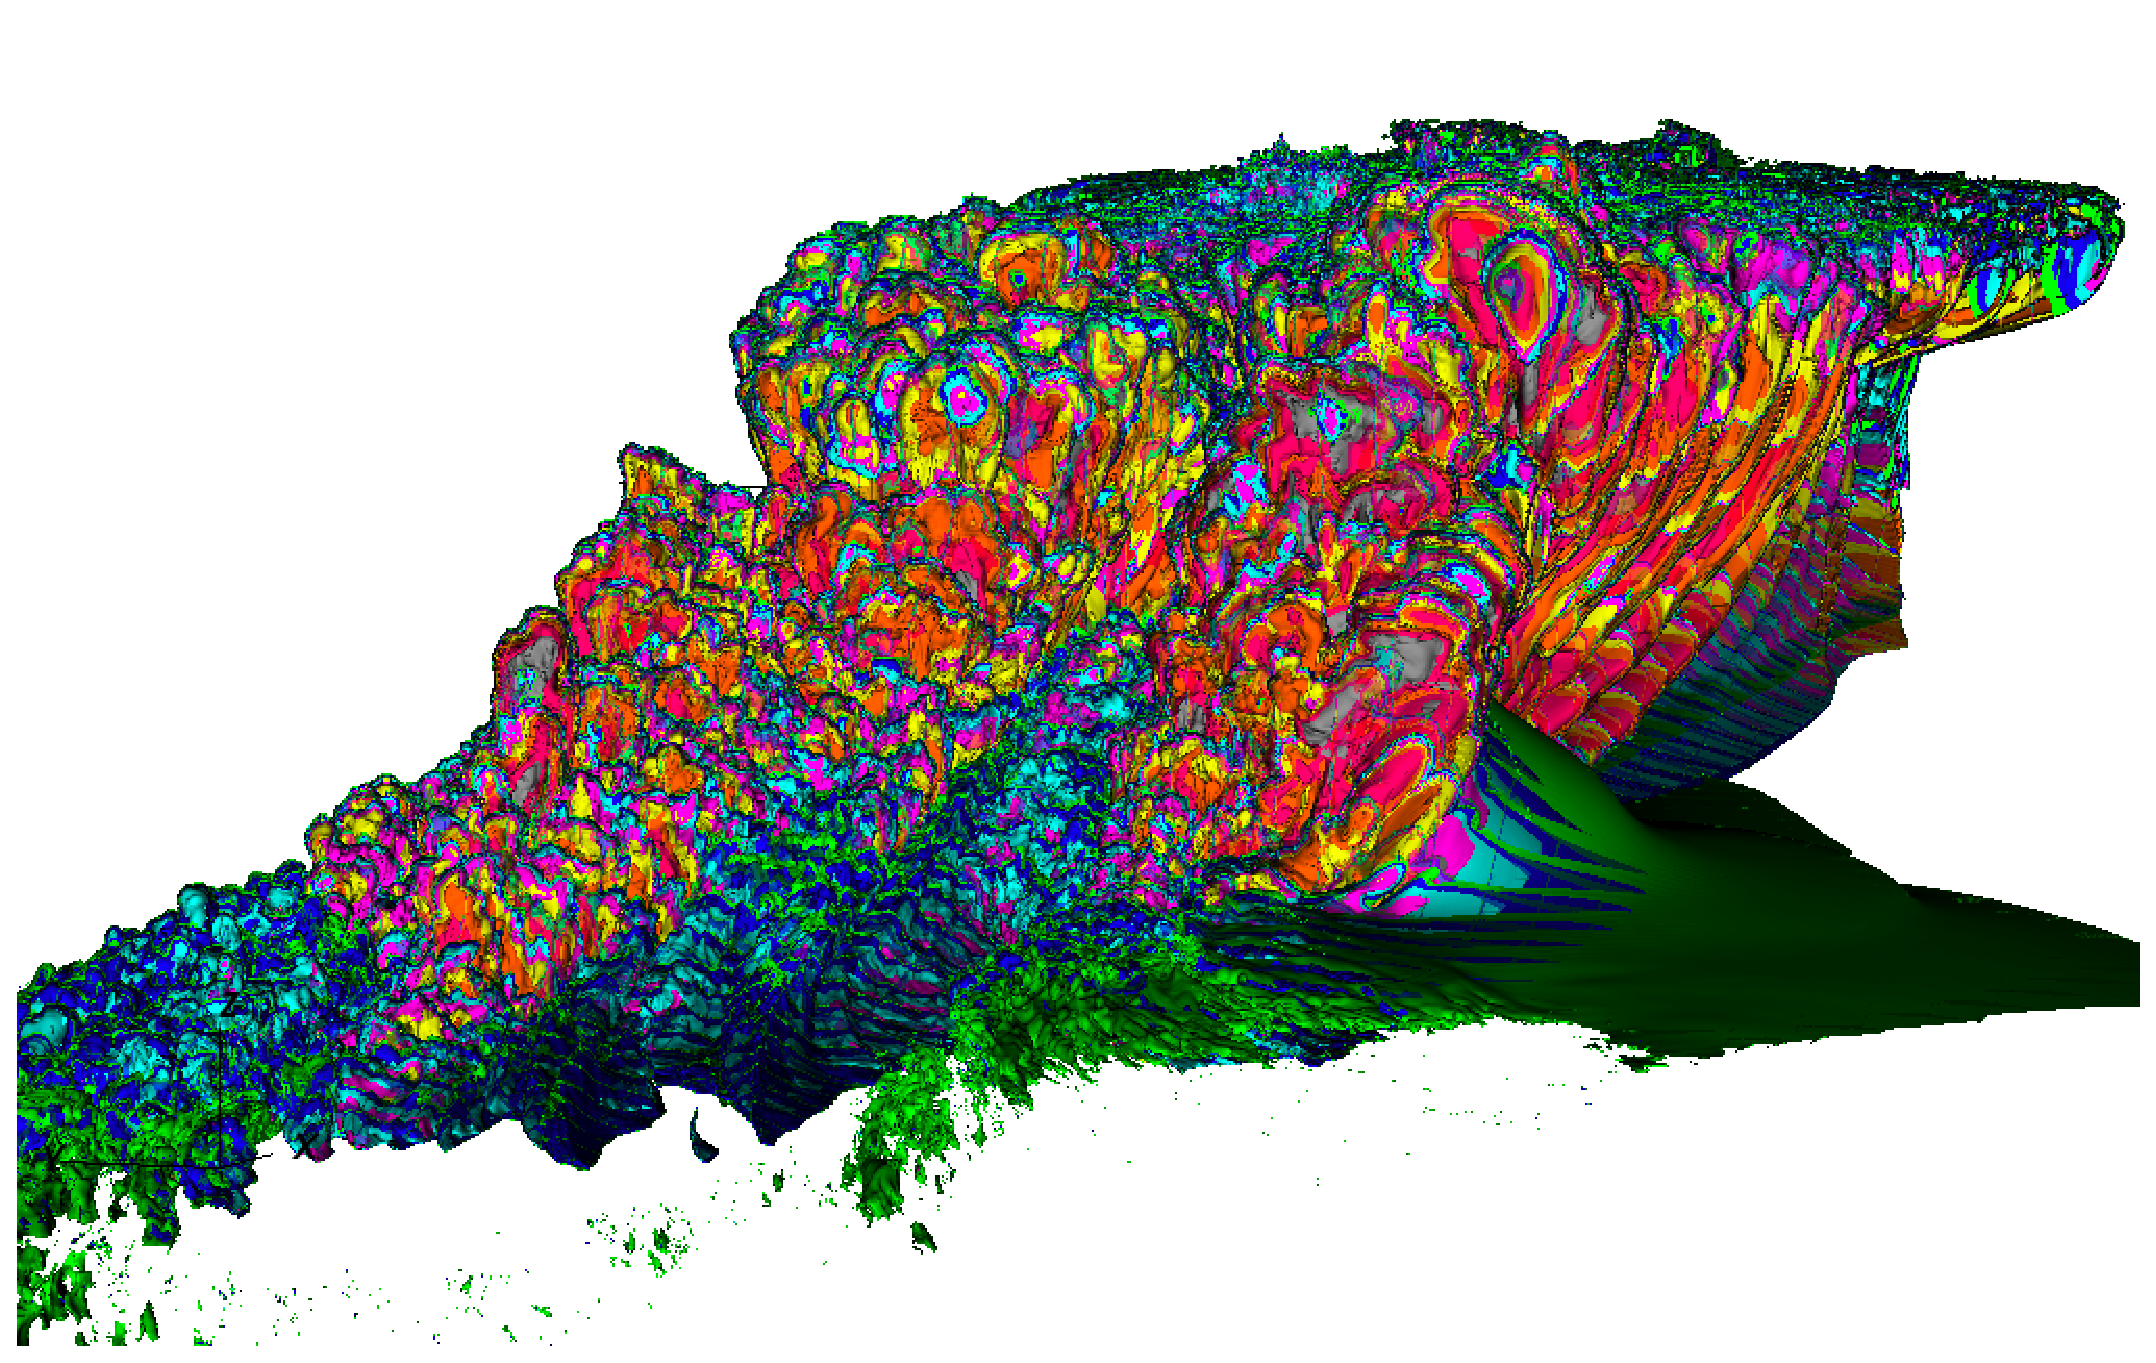
\includegraphics[width=3.5cm,height=3.5cm]{figures/cm1-isosurface.eps}}}
	\subfigure[CM1 Ray Casting]{
	\fbox{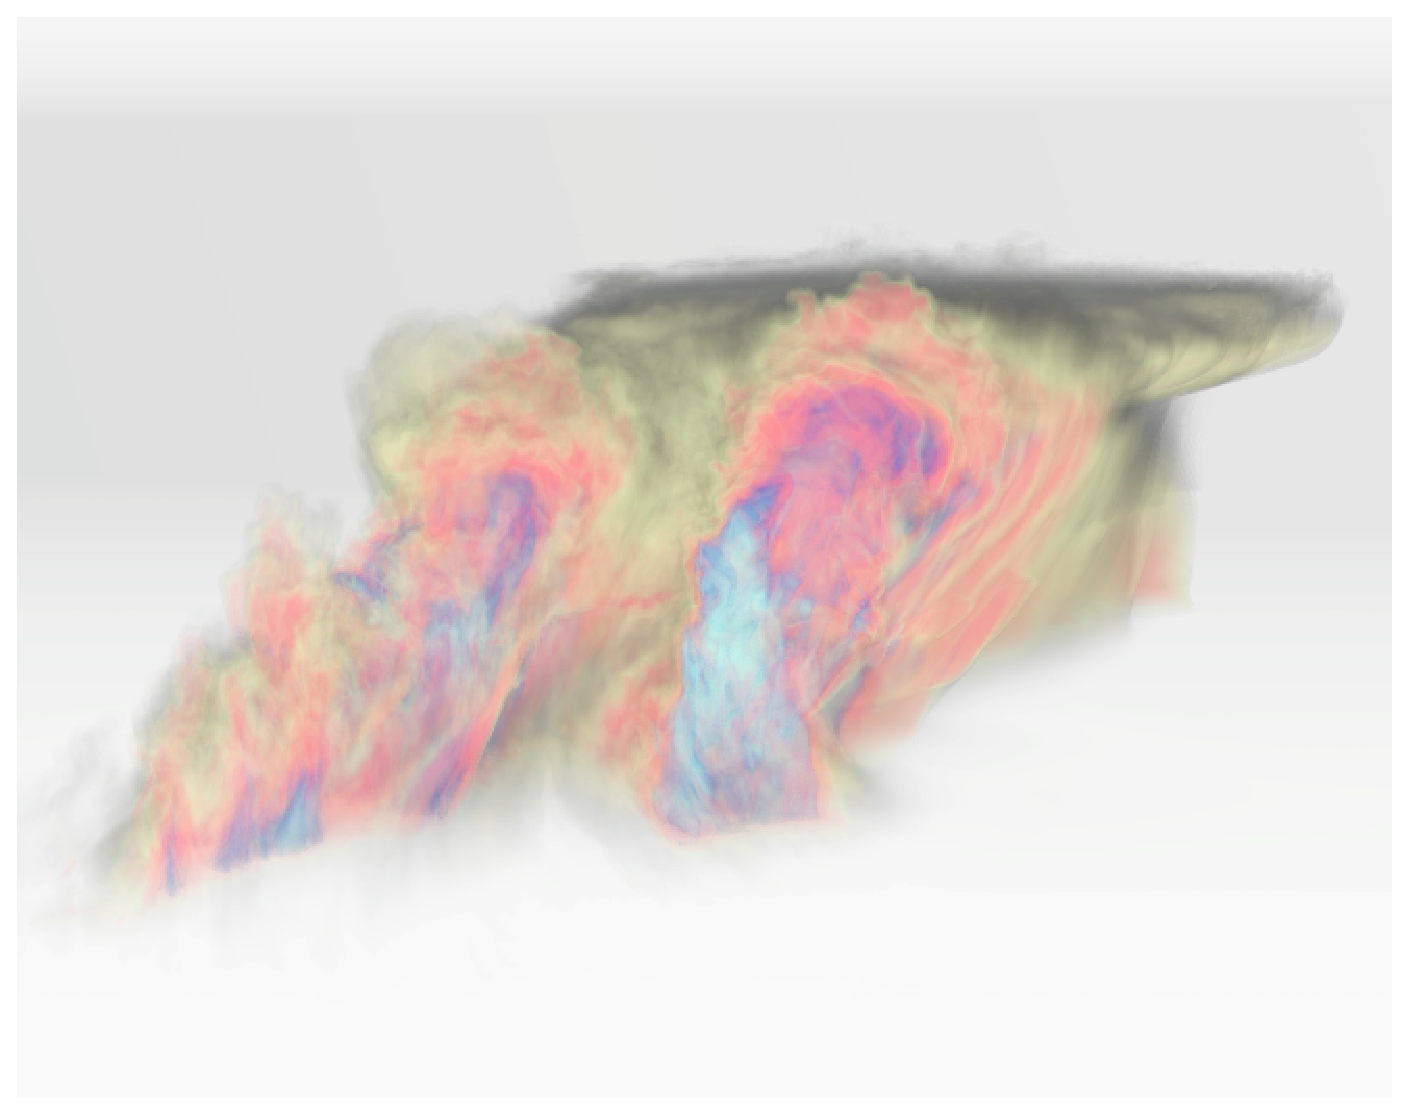
\includegraphics[width=3.5cm,height=3.5cm]{figures/cm1-raycasting.eps}}}
	\subfigure[Nek5000 Isosurface]{
	\fbox{\includegraphics[width=3.5cm,height=3.5cm]{figures/nek5-volume.eps}}}
	
	\caption{Example results obtained in situ with Damaris:
	(a) 10-level isosurface of the DBZ variable on 6400 cores (Blue Waters).
	(b) Ray-casting of the \emph{dbz} variable on 6400 cores (Blue Waters).
	(c) Ten-level isosurface of the $y$ velocity field in 
	the TurbChannel configuration of Nek5000.}\label{fig:visualresults}
\end{figure}

\subsubsection{Impact of Dedicated Cores on the Scalability of Visualization Tasks}

With CM1 on Blue Waters, we measured the time (average of 15 
iterations) to complete either an isosurface rendering or a ray casting
rendering using time partitioning and dedicated cores for each scenario. 
The comparative results are reported in Figure~\ref{fig:cm1vistime}.

\begin{figure}[t]
\centering
	\subfigure[In Situ Isosurface]{
	\includegraphics[width=5.5cm]{figures/cm1-in-situ-isosurface.eps}}
	\quad
	\subfigure[In Situ Ray Casting]{
	\includegraphics[width=5.5cm]{figures/cm1-in-situ-ray-casting.eps}}
	\caption{Rendering time using ray-casting and isosurfaces, with 
	time-partitioning and dedicated cores with CM1. Note that the number of cores 
	represents the total number used for the experiments; using a dedicated-core 
	approach, 1/16 of this total number is effectively used for in situ visualization,
	which explains the overall higher rendering time with dedicated cores.}
	\label{fig:cm1vistime}
\end{figure}

The isosurface algorithm (resulting image presented in Figure~\ref{fig:visualresults} (a))
scales well with the number of cores 
using both approaches. A time-partitioning approach would thus be 
appropriate if the user does not need to hide the run time impact of in situ 
visualization.
However, on 6400 cores, it takes as much time 
to complete the rendering as on 400 dedicated cores. In
terms of pure computational efficiency, an approach based on dedicated cores is thus 16 
times more efficient.

The ray-casting algorithm (resulting image presented in Figure~\ref{fig:visualresults} (b))
on the other hand has a poorer scalability. After 
decreasing, the rendering time goes up again at a 6400-core scale, and it 
becomes about twice more efficient to use a reduced number of dedicated 
cores to complete this same rendering.

\paragraph{Conclusion} The choice of using dedicated cores versus a time-partitioning in situ visualization approach 
depends on (1) the intended visualization scenario, (2) the scale of the experiments and 
(3) the intended frequency of visual output. Our experiments show that at small scale,
the performance of rendering algorithms are good enough to be executed in a time-partitioning manner,
provided that the user is ready to increase the run time of his simulation. At large scale however,
it becomes more efficient to use dedicated cores, especially when using ray-casting,
where the observed rendering performance is substantially better when using a reduced number of
processes.

\subsubsection{Impact of In Situ Visualization on Run Time Variability}

Our goal in this series of experiments is to show the impact of in situ visualization
tasks on the run-time variability of the simulation, and to show how dedicated cores
help alleviate this variability. We show in particular the effect of 
interactivity on this variability. We use Nek5000 for this purpose.
 
Figure~\ref{fig:visualresults}~(c) shows the result of a 10-level 
isosurface rendering of the fluid velocity along the $y$ axis, with the 
TurbChannel case. We use the MATiS configuration to show the scalability of our 
approach based on Damaris against a standard, time-partitioning approach.

\paragraph{Results with the TurbChannel Configuration}
To assess the impact of in situ visualization on the run time, we run 
TurbChannel on 48 cores using the two approaches: first we use a 
time-partitioning mode, in which all 48 cores are used by the simulation and 
synchronously perform in situ visualization. Then we switch on one dedicated core per node,
leading to 46 cores being used by the simulation while 2 cores asynchronously run 
the in situ visualization tasks.

In each case, we consider four scenarios: 
\begin{enumerate}
	\item The simulation runs without visualization;
	\item A user connects VisIt to the simulation but does not ask for any output;
	\item The user asks for isosurfaces of the velocity fields but does not interact with VisIt any further 
	(letting the Damaris/Viz update the output after each iteration);
	\item The user has heavy interactions with the simulations (for example rendering different variables, 
using different algorithms, zooming on particular domains, changing the 
resolution).
\end{enumerate}

Figure~\ref{fig:nek5variability} presents a trace of the duration of each
iteration during the four aforementioned scenarios using the two approaches.
Figure~\ref{fig:nek5variability}~(a) shows that in situ visualization using 
a time-partitioning approach has a large impact on the 
simulation run time, even when no interaction is performed. The simple act of connecting
VisIt without rendering anything forces the simulation to at least update metadata at each iteration,
which takes time.
Figure~\ref{fig:nek5variability}~(b) shows that in situ visualization based on dedicated cores, 
on the other hand, is completely transparent from the point of view of the simulation.

\begin{figure}[t]
\centering
	\subfigure[Time-Partitioning]{
	\includegraphics[width=5.5cm]{figures/turbchannel-time-partitioning.eps}}
	\quad
	\subfigure[Dedicated Cores]{
	\includegraphics[width=5.5cm]{figures/turbchannel-space-partitioning.eps}}
	\caption[Run-time variability in CM1 due to in situ visualization]{Variability 
	in run time induced by different scenarios of in situ 
	interactive visualization.}\label{fig:nek5variability}
\end{figure}

\paragraph{Results with the MATiS Configuration}
We ran the MATiS configuration on 816 cores of the \emph{stremi} cluster. Each 
iteration takes approximately one minute and due to the size of the
mesh, it is difficult to perform interactive visualization. 
Therefore we connect VisIt and simply query for a 3D pseudo-color plot of the $vx$ 
variable ($x$ component of the fluid velocity) that is then continuously updated.
For the following results, the time-partitioning approach outputs one image every time step,
while dedicated cores adapted the output frequency to one image every 25 
time steps in order to avoid blocking the simulation when the shared memory buffer becomes full.

Figure~\ref{fig:matisruntime} reports the behavior of the application with and 
without visualization performed, and with and without dedicated cores. 
Corresponding statistics are presented in Table~\ref{tab:matisstats}.

\begin{figure}[t]
\centering
	\subfigure[Time Partitioning, Without Visualization]{
	\includegraphics[width=5.5cm]{figures/matis-tp-no-viz.eps}}
	\quad
	\subfigure[Time Partitioning, With Visualization]{
	\includegraphics[width=5.5cm]{figures/matis-tp-viz.eps}}
	\subfigure[Space Partitioning, Without Visualization]{
	\includegraphics[width=5.5cm]{figures/matis-sp-no-viz.eps}}
	\quad
	\subfigure[Space Partitioning, With Visualization]{
	\includegraphics[width=5.5cm]{figures/matis-sp-viz.eps}}
	\caption[Iteration time of Nek5000's MATiS configuration with and without in situ visualization]{Iteration time 
	of the MATiS configuration without visualization 
	(left) and with visualization enabled (right).
	Top: with time partitioning, visualization time adds to the simulation time. 
	Bottom: With dedicated cores, visualization time entirely overlaps with simulation time.}\label{fig:matisruntime}
\end{figure}

\begin{table}
	\center
\caption[Average iteration time of Nek5000's MATiS configuration]{Average 
	iteration time of the Nek5000 MATiS configuration with a
   time-partitioning approach and with dedicated cores, with and without 
   visualization.\vspace{0.5cm}}\label{tab:matisstats}
   \begin{tabular}{|l|l|c|c|}
   \hline
\textbf{Iteration Time} & & Average & Std. dev. \\
	\hline
\multirow{2}{*}{Time Partitioning} & w/o vis. & 75.07 sec  & 22,93 \\
	& with vis. & 205.21 sec & 57.15 \\
	\hline
\multirow{2}{*}{Space Partitioning} & w/o vis. & 67.76 sec & 20.09 \\
	& with vis. & 64.79 sec  & 20.44 \\
	\hline
   \end{tabular}
\end{table}

\paragraph{Conclusion} Time-partitioning visualization not only increases the average run time but 
also increases the standard deviation of this run time, making it more unpredictable.
On the other hand, the approach based on dedicated cores yields more consistent results.
One might expect dedicated cores to interfere with the
simulation as it performs intensive communications while the simulation runs. 
However, in practice we observe very little such run time variation.

We also remark that decreasing the number of cores used by the simulation can actually
decreases its run time. For instance with Nek5000 on Grid'5000, the simulation reaches the
limit of its scalability. Yet due to its memory requirements and the amount of memory available
in each node of this platform, it is still necessary to run
it on this number of nodes. In other words, as reducing the number of cores per node
actually used by the simulation increases its performance, it further motivates the
use of these spare cores for extra tasks such as visualization.

Finally, while the time-partitioning approach performs visualization at every 
time step here, dedicated cores have adapted the frequency of 
its output to 1 image every 25 time steps.
If a time-partitioning approach were to only output 1 image every 25 time steps 
(which corresponds to having only the $25^{th}$ iteration being impacted 
in Figure~\ref{fig:matisruntime} (b)), the completion time for 25 time steps 
would be 2007 seconds on average.
With dedicated cores, this takes 1620 seconds, that is, a 20\% speedup. 
Furthermore, since dedicated cores enable the visualization and 
simulation tasks to overlap, the total run time is unchanged with the addition of in situ visualization.
